\chapter*{Introduction}
% inspired from http://stackoverflow.com/questions/2488681/latex-unnumbered-section-in-header-of-document/2492571#2492571 
\markboth{\MakeUppercase{Introduction}}{}
%\addcontentsline{toc}{chapter}{Introduction}

\chaptquote{Neil Armstrong}{That's one small step for a man, one giant leap for mankind.}

Kerbal Space Program \cite{ksp} is a rocket simulation game; it lets
you build, launch and pilot a rocket to put up satellites, send probes,
land rovers, and have Kerbals do SCIENCE.

\begin{figure}[H]
	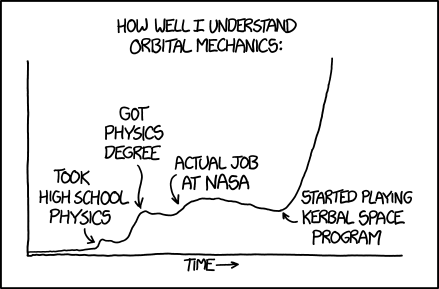
\includegraphics{img/xkcd1356.png}
	\caption{
		Mouseover text reads ”To be fair, my job at NASA was
		working on robots and didn't actually involve any orbital
		mechanics. The small positive slope over that period is
		because it turns out that if you hang around at NASA,
		you get in a lot of conversations about space.”
		\cite{xkcd1356}
	}
\end{figure}

A big advantage a KSP player has over actual rocket crafters is that she
can have rockets exploding without having to worry about consequences.
Half the fun of the game comes from finding out why your next rocket
will fail; thus, I urge you roll rockets to the launchpad early and not
bother thinking of every little thing that could go wrong.

AIRSICK will not cover the initiation to the game, since the interface is
specific to the game and prone to change. The game offers an intuitive
way to assemble rockets and has a handy interface to control the
flight. Rather, it will expose, explain and detail real principles of
physics that the game mimics. This information can be read simply for
curiosity, or can serve to design more precise launches in the game. When
possible, example values will be taken from reality or KSP.

\begin{remark}
KSP is a propietary software. You can play the demo for free, but will
be limited to an older version with only a few parts available for
building. The demo is way harder and the complete game way richer.
\end{remark}

\begin{important}
This document is intended to provide information both for beginners and
actual physicists. The first few chapters are an introduction to the
elementary concepts used within this book. In every chapters accurate
derivations and complete proofs are developed wherevever needed. If you
are not interested in the specifics of a demonstration or have already
some knowledge of basics physics, feel free to skip irrelevant parts.
\end{important}

\section*{Credits}

This document makes extensive use of pictures, diagrams and various
illustrations. Most figures were generated with the file from \LaTeX
using the Tikz package. When an external image was included as a figure,
a reference to the source is linked in the caption (e.g. \cite{xkcd1356}).

The image on the front cover \cite{3kerbalmun} and the chapter banners
\cite{banners} are KSP fan arts; the last illustration is a wallpaper
available on the official website of the game \cite{ksp}.
